\section{觀念與公式}

\subsection{基本概念}
向量表示大小與方向。\\
\textbf{定義}:
\begin{itemize}
    \item 幾何向量:箭頭表示。
    \item 坐標向量:$\vec{v} = (x, y)$。
    \item 模:$|\vec{v}| = \sqrt{x^2 + y^2}$。
\end{itemize}
\textbf{應用}:位置表示。\\
\textbf{大學技巧}:線性空間定義。

\subsection{向量運算}
基本運算規則。\\
\textbf{公式}:
\begin{itemize}
    \item 加法:$\vec{a} + \vec{b} = (a_1 + b_1, a_2 + b_2)$。
    \item 減法:$\vec{a} - \vec{b} = (a_1 - b_1, a_2 - b_2)$。
    \item 數乘:$k\vec{a} = (ka_1, ka_2)$。
    \item 內積:$\vec{a} \cdot \vec{b} = a_1 b_1 + a_2 b_2 = |\vec{a}| |\vec{b}| \cos \theta$。
\end{itemize}
\textbf{應用}:方向與大小。\\
\textbf{大學技巧}:矩陣表示。

\subsection{向量性質}
幾何與代數性質。\\
\textbf{性質}:
\begin{itemize}
    \item 平行:$\vec{a} = k\vec{b}$。
    \item 垂直:$\vec{a} \cdot \vec{b} = 0$。
    \item 單位向量:$\hat{v} = \frac{\vec{v}}{|\vec{v}|}$。
\end{itemize}
\textbf{應用}:夾角計算。\\
\textbf{大學技巧}:投影。

\subsection{幾何應用}
向量在平面幾何中應用。\\
\textbf{公式}:
\begin{itemize}
    \item 中點向量:$\vec{M} = \frac{\vec{A} + \vec{B}}{2}$。
    \item 三角形面積:$S = \frac{1}{2} |\vec{a} \cdot \vec{b} \sin \theta|$(或行列式)。
\end{itemize}
\textbf{應用}:物理與測量。\\
\textbf{大學技巧}:外積$|\vec{a} \times \vec{b}|$。

\section{例題解析}

\subsection{例題1:基本運算}
$\vec{a} = (3, 4)$,$\vec{b} = (1, -2)$,求$\vec{a} + \vec{b}$與$|\vec{a}|$。\\
\textbf{解}:$\vec{a} + \vec{b} = (4, 2)$,$|\vec{a}| = \sqrt{3^2 + 4^2} = 5$。

\subsection{例題2:內積與夾角}
$\vec{a} = (1, 2)$,$\vec{b} = (3, -1)$,求$\vec{a} \cdot \vec{b}$與夾角。\\
\textbf{解}:$\vec{a} \cdot \vec{b} = 1 \cdot 3 + 2 \cdot (-1) = 1$。\\
$|\vec{a}| = \sqrt{5}$,$|\vec{b}| = \sqrt{10}$,$\cos \theta = \frac{1}{\sqrt{50}}$,$\theta = \cos^{-1}\left(\frac{1}{5\sqrt{2}}\right)$。

\subsection{例題3:平行與垂直}
判斷$\vec{a} = (2, -4)$與$\vec{b} = (-1, 2)$是否平行。\\
\textbf{解}:$\vec{a} = -2\vec{b}$,平行。

\subsection{例題4:幾何應用}
點$A(1, 1)$,$B(3, 5)$,求中點向量與$AB$長度。\\
\textbf{解}:$\vec{AB} = (2, 4)$,中點$\vec{M} = (2, 3)$,$|\vec{AB}| = \sqrt{20} = 2\sqrt{5}$。

\subsection{例題5:應用題}
力$\vec{F} = (3, 4)$沿$\vec{d} = (1, 1)$分解,求分量。\\
\textbf{解}:投影$|\vec{F}| \cos \theta = \frac{\vec{F} \cdot \vec{d}}{|\vec{d}|} = \frac{7}{\sqrt{2}}$,分量$\frac{7}{\sqrt{2}} \cdot \frac{\vec{d}}{|\vec{d}|} = \left(\frac{7}{2}, \frac{7}{2}\right)$。

\section{圖形展示}
向量加法:
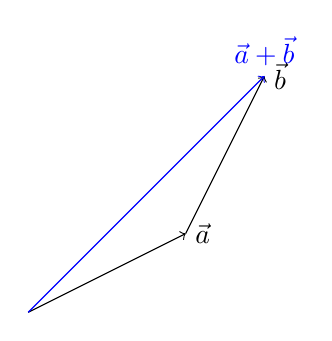
\begin{tikzpicture}
    \draw[->] (0,0) -- (2,1) node[right] {$\vec{a}$};
    \draw[->] (2,1) -- (3,3) node[right] {$\vec{b}$};
    \draw[->, blue] (0,0) -- (3,3) node[above] {$\vec{a} + \vec{b}$};
\end{tikzpicture}

\section{題庫}
\begin{enumerate}[label=\arabic*.]
    % 計算題 (10)
    \item $\vec{a} = (2, 3)$,求$|\vec{a}|$。
    \item $\vec{a} = (1, -1)$,$\vec{b} = (2, 3)$,求$\vec{a} + \vec{b}$。
    \item $\vec{a} = (4, 0)$,求$2\vec{a}$。
    \item $\vec{a} = (3, 4)$,$\vec{b} = (-1, 2)$,求$\vec{a} \cdot \vec{b}$。
    \item $\vec{a} = (1, 1)$,求單位向量。
    \item $\vec{a} = (5, -2)$,求$|\vec{a}|$。
    \item $\vec{a} = (2, -1)$,$\vec{b} = (1, 2)$,求$\vec{a} - \vec{b}$。
    \item $\vec{a} = (0, 3)$,$\vec{b} = (4, 0)$,求夾角。
    \item $\vec{a} = (6, 8)$,求$|\vec{a}|$。
    \item $\vec{a} = (1, 2)$,$\vec{b} = (-2, 1)$,求$\vec{a} \cdot \vec{b}$。
    % 應用題 (20)
    \item $\vec{a} = (3, 1)$,$\vec{b} = (2, -2)$,求$\vec{a} + \vec{b}$與夾角。
    \item 點$A(2, 3)$,$B(5, 7)$,求$\vec{AB}$與長度。
    \item $\vec{a} = (1, 3)$,$\vec{b} = (-3, 9)$,判斷是否平行。
    \item $\vec{a} = (2, 1)$,$\vec{b} = (-1, 2)$,求是否垂直。
    \item 力$\vec{F} = (4, 3)$沿$\vec{d} = (1, 0)$,求分量。
    \item $\triangle ABC$,$A(0, 0)$,$B(2, 0)$,$C(1, 3)$,求面積。
    \item $\vec{a} = (5, 2)$,$\vec{b} = (1, -1)$,求$\vec{a} \cdot \vec{b}$與$\theta$。
    \item 點$P(1, 2)$,$Q(4, 6)$,求中點向量。
    \item $\vec{a} = (3, -2)$,分解成$\vec{b} = (1, 1)$方向的分量。
    \item $\vec{a} = (4, 0)$,$\vec{b} = (0, 3)$,求面積。
    \item $\vec{a} = (2, 5)$,$\vec{b} = (-1, 2)$,求$|\vec{a} + \vec{b}|$。
    \item 點$A(0, 1)$,$B(3, 4)$,求$|\vec{AB}|$。
    \item $\vec{a} = (1, -1)$,$\vec{b} = (2, 2)$,求夾角。
    \item $\vec{F} = (6, 8)$沿$\vec{d} = (3, 4)$,求分量大小。
    \item $\triangle ABC$,$A(1, 1)$,$B(3, 2)$,$C(2, 4)$,求面積。
    \item $\vec{a} = (2, -3)$,$\vec{b} = (4, 1)$,求$\vec{a} - \vec{b}$。
    \item 點$P(0, 0)$,$Q(2, 3)$,$R(4, 1)$,求$\vec{PQ} + \vec{PR}$。
    \item $\vec{a} = (5, 0)$,$\vec{b} = (0, 5)$,求是否垂直。
    \item $\vec{a} = (3, 4)$,求單位向量。
    \item $\vec{a} = (1, 2)$,$\vec{b} = (3, -1)$,求$2\vec{a} - \vec{b}$。
    % 觀念題 (10)
    \item 向量模的意義?
    \item 內積如何判斷垂直?
    \item 平行向量的條件?
    \item 向量加法的幾何意義?
    \item 單位向量的定義?
    \item 內積與夾角的關係?
    \item 如何用向量求面積?
    \item 數乘向量的效果?
    \item 向量分解的原理?
    \item 中點向量的公式?
    % 進階題 (10)
    \item $\vec{a} = (2, 3)$,$\vec{b} = (1, -2)$,求投影分量於$\vec{b}$。
    \item $\triangle ABC$,$A(0, 0)$,$B(4, 0)$,$C(2, 3)$,求面積。
    \item $\vec{a} = (3, 1)$,$\vec{b} = (-2, 4)$,求$\theta$。
    \item $\vec{a} = (5, 2)$,分解成$\vec{b} = (1, 1)$與垂直分量。
    \item $\vec{a} = (1, 1)$,$\vec{b} = (2, -2)$,求$|\vec{a} + \vec{b}|$。
    \item 點$A(1, 2)$,$B(3, 5)$,$C(4, 1)$,求$\vec{AB} \cdot \vec{AC}$。
    \item $\vec{a} = (4, -3)$,$\vec{b} = (2, 1)$,求面積。
    \item $\vec{F} = (6, 8)$沿$\vec{d} = (1, 0)$,求分量與垂直分量。
    \item $\vec{a} = (2, 5)$,$\vec{b} = (-1, 3)$,求$3\vec{a} - 2\vec{b}$。
    \item $\triangle ABC$,$A(0, 0)$,$B(2, 2)$,$C(4, 0)$,求中點$M$向量。
    % 挑戰題 (10)
    \item $\vec{a} = (3, 4)$,$\vec{b} = (1, -1)$,求$\vec{a}$在$\vec{b}$上的投影向量。
    \item $\triangle ABC$,$A(0, 0)$,$B(3, 0)$,$C(0, 4)$,求面積與$\vec{AC}$單位向量。
    \item $\vec{a} = (2, 1)$,$\vec{b} = (-1, 2)$,求$\vec{a} + \vec{b}$與面積。
    \item $\vec{F} = (5, 5)$分解成$\vec{d} = (1, 0)$與垂直分量。
    \item 點$A(1, 1)$,$B(4, 3)$,$C(2, 5)$,求面積。
    \item $\vec{a} = (3, -2)$,$\vec{b} = (4, 1)$,求$\vec{a} \cdot \vec{b}$與$\theta$。
    \item $\vec{a} = (1, 2)$,$\vec{b} = (2, 1)$,求$|\vec{a} - \vec{b}|$與夾角。
    \item $\triangle ABC$,$A(0, 0)$,$B(5, 0)$,$C(2, 4)$,求面積。
    \item $\vec{a} = (4, 3)$,$\vec{b} = (-2, 5)$,求投影與垂直分量於$\vec{b}$。
    \item 點$P(0, 0)$,$Q(2, 3)$,$R(4, 1)$,求$\vec{PQ} \cdot \vec{PR}$。
\end{enumerate}